\documentclass[10pt,a4paper,table]{article}
	
	\usepackage{amsmath,amssymb,amsthm,mathtools,amsfonts}
	\usepackage{breqn}
	\usepackage[utf8]{inputenc}
	\usepackage[danish]{babel}
	\usepackage[T1]{fontenc}
	
	%%%%%%%%%%%%%%%%%%%%%%%%%%%%%%%%%%%%%%%%%%%%%%%%%%%%%%%%%%%%%%%%%%%%%%%%%%%%%% Fonts
	
	\usepackage{fontspec}
	\setmainfont{Times New Roman}
	\newfontfamily\garamond[Numbers=OldStyle]{EB Garamond}
	\newfontfamily\plantin[Numbers=OldStyle]{Plantin MT Pro}
	\newfontfamily\wal{Walbaum Com}
	\newfontfamily\klav{Klavika}
	\newfontfamily\klavl{Klavika light}
	\newfontfamily\quotefont[Ligatures=TeX]{Linux Libertine O}
	\newfontfamily\vest{TRY Vesterbro Regular}
	\newfontfamily\vestb{TRY Vesterbro Poster}
	\newfontfamily\overp{Overpass}
	
	%%%%%%%%%%%%%%%%%%%%%%%%%%%%%%%%%%%%%%%%%%%%%%%%%%%%%%%%%%%%%%%%%%%%%%%%%%%%%% Colors
	
	\usepackage{xcolor}
	\usepackage{transparent}
	
	\definecolor{frbblue}{RGB}{47, 88, 109}
	\definecolor{hgred}{RGB}{140, 10, 10}
	\definecolor{frbgreenl}{RGB}{162, 202, 137}
	\definecolor{frbgreen}{RGB}{28, 85, 66}
	\definecolor{frbgrey}{RGB}{243, 245, 242}
	
	%%%%%%%%%%%%%%%%%%%%%%%%%%%%%%%%%%%%%%%%%%%%%%%%%%%%%%%%%%%%%%%%%%%%%%%%%%%%%% Other Graphics
	
	\usepackage{graphicx}
	\graphicspath{{../img/}}
	\usepackage{tikz}
	\usetikzlibrary{calc}
	\usepackage{placeins}
	
	\usepackage[pdfborder={0 0 0}]{hyperref} %% Ingen firkant rundt om referencer

	\usepackage{multicol}
	\usepackage{cellspace}
		\setlength\cellspacetoplimit{100pt}
		\setlength\cellspacebottomlimit{100pt}
	\usepackage{tabularx}
		\newcolumntype{b}{>{\hsize=\hsize}>{\centering\arraybackslash}X}
	\usepackage{siunitx}
	\usepackage{cellspace}
		\setlength\cellspacetoplimit{4pt}
		\setlength\cellspacebottomlimit{4pt}
	
	\usepackage{enumitem}% better controls with enumerating
	\usepackage{wrapfig}
	\usepackage{caption}
	%\usepackage{dirtytalk}
	%\usepackage{tasks}
	\usepackage{titlesec}

	\setlength{\parskip}{0.5\baselineskip}
	\setlength{\parindent}{0cm}
	\setlist[enumerate]{label=\alph*),left=20pt}
	%\setlist[enumerate]{leftmargin=\parindent}
	%\setlist[enumerate]{nosep}
	
	
	%%%%%%%%%%%%%%%%%%%%%%%%%%%%%%%%%%%%%%%%%%%%%%%%%%%%%%%%%%%%%%%%%%%%%%%%%%%%%% New commands
	
	\newcommand\svar[1]{\newline\textcolor{red}{\textbf{Svar}\\#1}}
	
	\usepackage[h]{esvect}
	\newcommand{\twvect}[2]{\ensuremath{\begin{pmatrix}#1\\#2\end{pmatrix}}}
	
	\newcommand*\quotesize{20}
	\newcommand*{\openquote}
		{\tikz[remember picture,overlay,xshift=-3ex,yshift=-0ex]
			\node (OQ) {\quotefont\fontsize{\quotesize}{\quotesize}\selectfont``};\kern0pt}

	\newcommand*{\closequote}[1]
		{\tikz[remember picture,overlay,xshift=2ex,yshift={#1}]
			\node (CQ) {\quotefont\fontsize{\quotesize}{\quotesize}\selectfont''};}
			
	\newcommand{\qm}[1]{``#1''}
	\newcommand{\iquote}[1]{\begin{quote}\itshape \openquote#1\hfill\closequote{0ex} \end{quote}}
	
	%%%%%%%%%%%%%%%%%%%%%%%%%%%%%%%%%%%%%%%%%%%%%%%%%%%%%%%%%%%%%%%%%%%%%%%%%%%%%% Sections
	\usepackage{chngcntr}
	
	\renewcommand\thesection{\arabic{section}}

	\titleformat{\section}[block] 
  		{\flushright\overp\Large\color{frbgreen}}    % format for whole title
  		{}                           % no separate label (empty)
  		{0pt}                        % spacing between label and title
		{DELPRØVE \thesection}       % prepend "Delprøve <number>"
		[{\color{frbgreenl}\vspace{-1em}\hspace*{-0.165\linewidth}\rule{\dimexpr1.165\linewidth\relax}{0.4pt}\kern1mm}]
	
	\counterwithout{subsection}{section}
	\renewcommand\thesubsection{Øvelse \arabic{subsection}}
	\titleformat{\subsection}[leftmargin]{\bfseries}{}{0pt}{\hspace{-5em}\thesubsection}
	
	%%%%%%%%%%%%%%%%%%%%%%%%%%%%%%%%%%%%%%%%%%%%%%%%%%%%%%%%%%%%%%%%%%%%%%%%%%%%%% Header & Footer
	
	\usepackage{bigfoot}
	\DeclareNewFootnote{a}
		\renewcommand{\thefootnotea}{\fnsymbol{footnotea}}
			\newcommand{\footnotes}[1]{\footnotea[2]{#1}} % here you can specify what symbol you want in footnotes
			\MakePerPage{footnotes}
	
		\usepackage{fancyhdr}
	\fancypagestyle{plain}{%
		\setlength{\headheight}{60pt}%
		\setlength{\headsep}{0pt}
		\fancyhf{}% No header/footer
		\renewcommand{\footrulewidth}{0pt}% No footer rule
		\renewcommand\headrule{}% No header rule
		\fancyhead[L]{}
		\fancyhead[C]{}
		\fancyhead[R]{\overp\color{frbgreenl}\normalsize \overp Mat C-B\\\huge\color{frbgreen}\vestb Differentialregning}
		\cfoot{\thepage}
	}
	\pagestyle{fancy}
	\fancyhf{}
	\renewcommand\headrule{}
	\lhead{}
	\rhead{}
	\cfoot{\thepage}
	
	%%%%%%%%%%%%%%%%%%%%%%%%%%%%%%%%%%%%%%%%%%%%%%%%%%%%%%%%%%%%%%%%%%%%%%%%%%%%%% Document

\begin{document}
\thispagestyle{plain}
\begin{tikzpicture}[remember picture,overlay]
    \node[anchor=north west,yshift=-48pt,xshift=120pt,opacity=0.2]%
        at (current page.north west)
        {\includegraphics[scale=0.25]{frbvuc_logo.png}};
\end{tikzpicture}
\begin{tikzpicture}[remember picture,overlay]
  % a light grey/green like in your screenshot
  \definecolor{bgline}{RGB}{205,214,208}

  % center for the circles (placed a bit *outside* the page to the left)
  \coordinate (C) at ($(current page.north)+(35mm,-5mm)$);

  % two thin concentric circles
  \draw[bgline, line width=0.6pt] (C) circle (65mm);

  % optional vertical hairlines near the page margins
  \draw[bgline, line width=0.4pt]
    ($(current page.north east)+(0,0mm)$) ++(-28mm,0)
    -- ($(current page.south east)+(0,10mm)$) ++(-28mm,0);
\end{tikzpicture}

\vspace{4em}

\subsection{}
Bestem de følgende funktionsværdier:
\begin{enumerate}
    \item $f(x) = 2x + 3, \quad f(4)$
    \item $g(x) = -x + 7, \quad g(2)$
    \item $h(x) = x^2 - 3x + 2, \quad h(1)$
    \item $p(x) = 3x^2 + 2x - 5, \quad p(-1)$
    \item $q(x) = (x-2)(x+3), \quad q(2)$
    \item $r(x) = \sqrt{x^2+7}, \quad r(11)$
    \item $s(x) = \tfrac{1}{x^2-5}, \quad s(3)$
    \item $t(x) = e^{0.5x} - x^2, \quad t(4.2)$
    \item $u(x) = \ln(x^2+1), \quad u(7)$
    \item $v(x) = x^2 + \sqrt{2x+5}, \quad v(12)$
\end{enumerate}

\subsection{}
Bestem den afledte funktion $f'(x)$ for hver af de følgende funktioner:

\begin{enumerate}
    \item $f(x) = 3x^5 - 2x^3 + 7x - 4$
    \item $f(x) = -x^6 + 4x^4 - 2x^2 + 9$
    \item $f(x) = 5x^7 - 8x^3 + 6$
    \item $f(x) = x^4 - 3x^2 + 2x - 1$
    \item $f(x) = -2x^9 + 6x^3 - 7$
    \item $f(x) = \sqrt{x} + 3x^2$
    \item $f(x) = \tfrac{1}{x} - 4x^3$
    \item $f(x) = e^x + 2x^2$
    \item $f(x) = \ln(x) + x^3$
    \item $f(x) = x^5 - \tfrac{7}{x} + \sqrt{x}$
\end{enumerate}

\subsection{}
Løs følgende ligninger.

\begin{enumerate}
    % Til hånden
    \item $2x + 5 = 11$
    \item $3x - 7 = 2x + 1$
    \item $x^2 - 5x + 6 = 0$
    \item $2x^2 + 3x - 2 = 0$
    \item $(x-2)(x+3) = 0$

    % Til CAS
    \item $x^3 - 2x^2 + x - 5 = 0$
    \item $x^4 - 3x^2 + 2 = 0$
    \item $e^x = 3x$
    \item $\ln(x) + x^2 = 4$
    \item $\sqrt{x+2} = x - 1$
\end{enumerate}

\subsection{}
Bestem følgende ved hjælp af differentialregning:

\begin{enumerate}
    \item Funktionen $f$ er givet ved
    $$
    f(x) = x^2 - 4x + 7.
    $$
    Bestem tangenthældningen i $x=2$.

    \item Funktionen $g$ er givet ved
    $$
    g(x) = 3x^2 + 2x - 1.
    $$
    Bestem en ligning for tangenten til grafen for $g$ i punktet $(1, g(1))$.

    \item Funktionen $h$ er givet ved
    $$
    h(x) = -x^3 + 6x^2 - 9x.
    $$
    Bestem monotoniforholdene for $h$.

    \item Funktionen $p$ er givet ved
    $$
    p(x) = \sqrt{x}, \quad x \geq 0.
    $$
    Bestem tangenthældningen i $x=4$.

    \item Funktionen $q$ er givet ved
    $$
    q(x) = 6x^8-x^4-x^3+5.
    $$
    Undersøg, om $q$ har vendetangent i $x=0$, og afgør om punktet er et ekstremum.
\end{enumerate}

\clearpage
\subsection{}
Husk følgende begreber

\begin{description}
    \item[Tangenthældning] Hældningen på den rette linje, der rører grafen i ét punkt. Fortæller hvor stejl grafen er netop dér.
    \item[Differentialkvotient] Den grænseværdi, der definerer den præcise hældning af tangenten i et punkt. Svarer til øjeblikkelig ændringshastighed.
    \item[Afledt funktion $f'(x)$] En funktion, der giver tangenthældningen i hvert punkt på grafen for $f$.
    \item[Monotoniforhold] Angiver hvor en funktion er voksende, aftagende eller konstant. Afgøres af fortegnet på $f'(x)$.
    \item[Ekstremum (maksimum/minimum)] Punkter hvor funktionen skifter fra at være voksende til aftagende (maksimum) eller omvendt (minimum). Finder man ofte ved at løse $f'(x)=0$.
    \item[Stationært punkt] Et punkt på grafen, hvor den afledte funktion er nul, dvs. steder med vandret vendetangent (inklusiv ekstrema).
    \item[Tangentligning] En ligning for en tangent i punktet $(x_0, f(x_0))$.
    \item[Differentiabel funktion] En funktion, der kan differentieres (dvs. har en veldefineret tangent) i det pågældende punkt eller interval.
    \item[Kontinuitet] Et krav om, at grafen kan tegnes uden “hop” – ofte en forudsætning for differentiabilitet.
    \item[Regneregler for differentiation]
\
        \begin{itemize}
            \item Sum- og differensregel: $(f \pm g)' = f' \pm g'$
            \item Konstantgangeregel: $(k\cdot f)' = k\cdot f'$
        \end{itemize}
    \item[Standardafledninger]
\
        \begin{itemize}
			\item $(x^a)' = a \cdot x^{a-1}$
            \item $(e^x)' = e^x$
            \item $(\ln(x))' = \tfrac{1}{x}$
            \item $(\sqrt{x})' = \tfrac{1}{2\sqrt{x}}$
            \item $\left(\tfrac{1}{x}\right)' = -\tfrac{1}{x^2}$
        \end{itemize}
    \item[Tretrinsreglen] Metode til at finde differentialkvotienten uden formel:
        \[
        f'(x_0) = \lim_{h \to 0} \frac{f(x_0+h)-f(x_0)}{h}.
        \]
\end{description}

\clearpage
\begin{tikzpicture}[remember picture,overlay]
    \node[anchor=south east,yshift=48pt,xshift=-40pt,opacity=0.1]%
        at (current page.south east)
        {\includegraphics[scale=0.25]{frbvuc_logo.png}};
\end{tikzpicture}
\pagestyle{empty}
\begin{tikzpicture}[remember picture,overlay]
  \draw[step=0.5cm,gray!50,very thin] (current page.south west) grid (current page.north east);
\end{tikzpicture}

\end{document}

%%%%%%%%%%%%%%%%%%%%%%%%%%%%%%%%%%%%%%%%%%%%%%%%%%%%%%%%%%%%%%%%%%%%%%%%%%%%%% Skabeloner

% Sidestillet figur
\begin{wrapfigure}[8]{r}{0.2\textwidth}
\vspace{-18pt}
\includegraphics[width=0.3\textwidth]{ovn}
\end{wrapfigure}

% Midterstillet figur
\begin{figure}[h!]
\centering
\includegraphics[width=0.8\textwidth]{abc}
\end{figure}

% Førstillet figur
\
\begin{figure}[h!]
\centering
\vspace{-15pt}
\includegraphics[width=0.35\textwidth]{stud}
\end{figure}

% Tabel
\begin{figure}[h!]
\centering\renewcommand{\arraystretch}{1.5}
\begin{tabularx}{0.9\textwidth}{|l|b|b|b|b|b|b|}
	\hline \cellcolor{hggreen} Decimaltal & 7\% & -51\% & 13,7\% & 126\% & 456\% & 0,28\%\\\hline
	\cellcolor{hggreen} Procenttal &  &  &  &  &  & \\\hline
\end{tabularx}
\end{figure}

% Forklaringsopgaver
\begin{align*}
&&	&						&&\underset{\rule{0.8\linewidth}{0pt}}{\textbf{Forklaring:}}\\[1em]
&&	&\frac{(x+2)^2 - 4}{x} 		&&\underset{\rule{0.8\linewidth}{0.4pt}}{\text{Udtrykket skrives op.}}\\[2em]
&&	=&\ \frac{x^2 + 4 + 4x - 4}{x}	&&\underset{\rule{0.8\linewidth}{0.4pt}}{\text{}}\\[2em]
&&	=&\ \frac{x^2 + 4x}{x}			&&\underset{\rule{0.8\linewidth}{0.4pt}}{\text{}}\\[2em]
&&	=&\ x + 4					&&\underset{\rule{0.8\linewidth}{0.4pt}}{\text{}}\\[2em]
\end{align*}

% Sørg for at figur er placeret før et vidst sted
\FloatBarrier




